\documentclass[12pt]{letter}
\usepackage{amsmath,amsfonts,amsthm,amstext,amssymb,graphicx, multicol,fancyhdr,lastpage,fullpage,framed,fancybox,enumerate,tikz,color,mathrsfs, polynom, pifont, stmaryrd}
\usepackage[margin=0.6in,headsep=3pt, headheight=15pt]{geometry}

% ----------------------------------------------------------
% Custom Definitions, Commands, Environments, etc.

% Sets of numbers
\def\R{\mathbb{R}} % The reals
\def\N{\mathbb{N}} % The naturals
\def\Z{\mathbb{Z}} % The integers
\def\Q{\mathbb{Q}} % The rationals
\def\C{\mathbb{C}} % The complex
\def\F{\mathbb{F}} % Field

% Blank space
\newcommand{\blank}[1]{\underline{\hspace{#1}}} % Blank space

% Change font colors
\newcommand{\cyan}[1]{{\color{cyan}{#1}}} % Changes font to cyan
\newcommand{\red}[1]{{\color{red}{#1}}} % Changes font to red
\newcommand{\magenta}[1]{{\color{magenta}{#1}}} % Changes font to magenta
\newcommand{\orange}[1]{{\color{orange}{#1}}} % Changes font to orange
\newcommand{\yellow}[1]{{\color{yellow}{#1}}} % Changes font to yellow
\newcommand{\violet}[1]{{\color{violet}{#1}}} % Changes font to violet
\newcommand{\green}[1]{{\color{green}{#1}}} % Changes font to green
\newcommand{\blue}[1]{{\color{blue}{#1}}} % Changes font to blue
\newcommand{\white}[1]{{\color{white}{#1}}} % Changes font to white

% Fitted inclusion symbols
\newcommand{\fp}[1]{\left({#1}\right)} % Fitted parentheses around content
\newcommand{\fb}[1]{\left[{#1}\right]} % Fitted brackets
\newcommand{\lhoi}[1]{\left({#1}\right]} % Left half-open interval
\newcommand{\rhoi}[1]{\left[{#1}\right)} % Right half-open interval
\newcommand{\set}[1]{\left\{{#1}\right\}} % Fitted braces (useful for sets)
\newcommand{\av}[1]{\left|{#1}\right|} % Fitted absolute value bars
\newcommand{\step}[1]{\left\llbracket {#1} \right\rrbracket}

% Augmented Matrix Environment
\newenvironment{amatrix}[1]{%
	\left[\begin{array}{@{}*{#1}{c}|c@{}}
	}{%
	\end{array}\right]
}

% Miscellaneous
\def\then{\Rightarrow}
\def\to{\rightarrow}
\def\d{^{\circ}}
\newcommand{\?}{\stackrel{?}{=}}
\newcommand{\cmark}{\text{ \ding{51}}}
\newcommand{\xmark}{\text{ \ding{55}}}



% Coordinate Plane (Four-Quadrant)
\def\coordplane {
	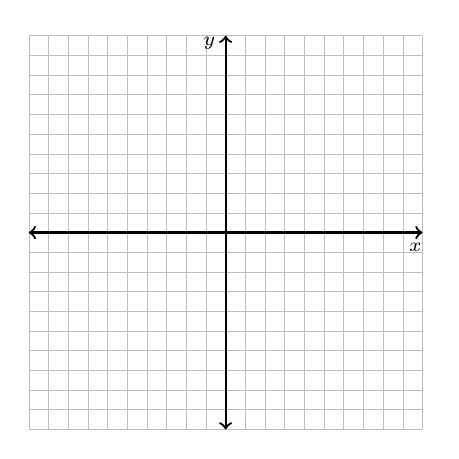
\begin{tikzpicture}        \draw[step=0.25cm,black,very thin,opacity=0.25] (-2.5cm, -2.5cm) grid (2.5cm, 2.5cm);
		\draw[<->,thick,black] (-2.5cm, 0) -- (2.5cm, 0) node[anchor=north west,pos=0.94,font=\scriptsize]{$x$};
		\draw[<->,thick,black] (0,-2.5cm) -- (0, 2.5cm) node[anchor=south east,font=\scriptsize,pos=0.94]{$y$};
	\end{tikzpicture}
}

% Coordinate Plane (One-Quadrant)
\def\onequad {
	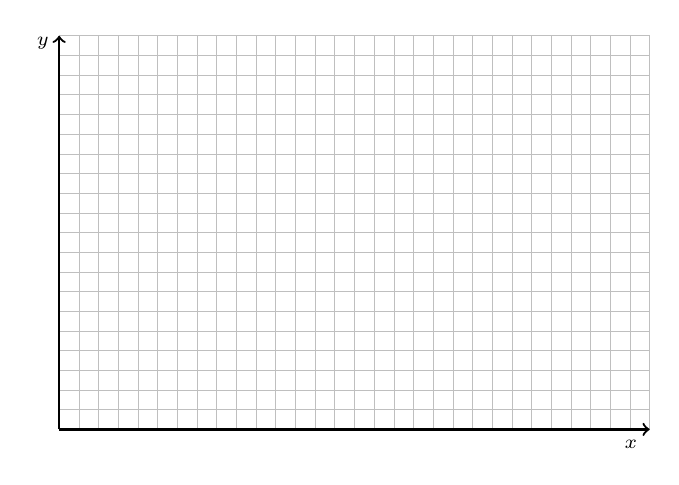
\begin{tikzpicture}
		\draw[step=0.25cm, black, very thin, opacity=0.25] (0,0) grid (7.5cm,5cm);
		\draw[->, thick, black] (0,0) -- (7.5cm, 0) node[anchor=north west,font=\scriptsize,pos=0.94]{$x$};
		\draw[->, black, thick] (0,0) -- (0,5cm) node[anchor=south east,font=\scriptsize,pos=0.94]{$y$};
	\end{tikzpicture}
}

% Counters
\newcounter{exercise}

% Exercise environment (auto-numbered)
\newenvironment{exercise}[1][]{\begin{framed}\refstepcounter{exercise}\textbf{Exercise~\theexercise:} #1}{\end{framed}}

% Book exercise environment
\newenvironment{bex}[2] {
	\begin{framed}
		\textbf{Book Exercise {#1}:} #2
	\end{framed}	
}
% ----------------------------------------------------------

% ----------------------------------------------------------
% Header and Footer Information
% \pagestyle{fancy}
% \fancyhf{}
% \renewcommand{\headrulewidth}{0pt}
% \rhead{Name: \blank{2in}}
% \lhead{@}
% \rfoot{Page \thepage \, of \,\pageref{LastPage}}
% ----------------------------------------------------------
\author{Jacob Ayers}

\begin{document}
	
	\textbf{Jacob Ayers \\ Assignment 11, Exercise \#14 \\ MAT 110 Spring 2021}
	
	\begin{exercise}
		According to Nielsen Media Research, of all the U.S. households that owned at least one television set, 83\% had two or more sets. A local cable company canvassing the town to promote a new cable service found that of the 300 randomly selected households visited, 240 had two or more television sets. At $\alpha = 0.05$, is there sufficient evidence to conclude that the proportion is less than the one in the report?
	\end{exercise}
	
	\textbf{Important Values} \\
	$p = 0.83$ \\ $q = 1 - 0.83 = 0.17$ \\ $\hat{p} = \frac{240}{300} = 0.80$ \\ $n = 300$ \\ $\alpha = 0.05$
	
	\textbf{Hypotheses} \\
	The null hypothesis states that there is no difference between the sample proportion and the reported population proportion.
	Thus the null hypothesis is $$H_0: p = 0.83.$$
	The claim here is that the proportion is \textit{less than} the one in the report.
	So the alternative hypothesis is $$H_1: p < 0.83.$$
	
	\textbf{Critical Value(s)} \\
	Since the alternative hypothesis is less than, this is a left-tailed test. Unfortunately, I can't figure out a good way to insert an image to illustrate here, but we need to find the $z$-value corresponding to an area of $0.0500$ to the left. This can be done using the standard normal table; the critical value is $z = -1.65$.
	
	\textit{Note:} This means that we will reject $H_0$ if the test value is less than $-1.65$, and not reject otherwise.
	
	\textbf{Test Value} \\
	$\dfrac{\hat{p} - p}{\sqrt{pq / n}} = \dfrac{0.80 - 0.83}{\sqrt{(0.83\cdot 0.17) / 300}} \approx -1.383$
	
	\textbf{Decision} \\
	Since $-1.383 > -1.65$ and is thus in the noncritical region, we should not reject $H_0$.
	
	\textbf{Summary} \\
	We are trying to conclude that the proportion is less than the one in the report. In other words, the claim is that $H_1$ is true. We didn't reject $H_0$, so we can't come to this conclusion. Sample summary:
	
	There is not sufficient evidence to conclude that the proportion is less than the one in the report.
	
\end{document}